\documentclass[]{book}
\usepackage{amsmath,amssymb}
\usepackage{amsthm}
\usepackage{xpatch}
\xpatchcmd\swappedhead{~}{.~}{}{}

\usepackage[T1]{fontenc}
\usepackage[utf8]{inputenc}

\usepackage{parskip}
\usepackage{lmodern}


\usepackage{xcolor}

\usepackage{hyperref}

\usepackage[ marginparwidth=3cm, marginparsep=0cm]{geometry}
\usepackage{graphicx}
\usepackage[spanish]{babel}


% Scale images if necessary, so that they will not overflow the page
% margins by default, and it is still possible to overwrite the defaults
% using explicit options in \includegraphics[width, height, ...]{}
\setkeys{Gin}{width=\maxwidth,height=\maxheight,keepaspectratio}
% Set default figure placement to htbp
\makeatletter
\def\fps@figure{htbp}
\makeatother


\providecommand{\tightlist}{%
  \setlength{\itemsep}{0pt}\setlength{\parskip}{0pt}}

  
%remove section numbers
%\setcounter{secnumdepth}{0}

\title{Introducción a la probabilidad}
\author{Hugo J. Bello}
\date{}


\renewcommand{\familydefault}{\sfdefault}
\setcounter{chapter}{2}


\theoremstyle{plain}
\swapnumbers % Switch number/label style
\newtheorem{theorem}{Theorem}[section]
\newtheorem{corollary}[theorem]{Corollary}
\newtheorem{lemma}[theorem]{Lemma}
\newtheorem{claim}{Claim}[theorem]
\newtheorem{axiom}[theorem]{Axiom}
\newtheorem{conjecture}[theorem]{Conjecture}
\newtheorem{fact}[theorem]{Fact}
\newtheorem{hypothesis}[theorem]{Hypothesis}
\newtheorem{assumption}[theorem]{Assumption}
\newtheorem{proposition}[theorem]{Proposition}
\newtheorem{property}[theorem]{Propiedad}
\newtheorem{properties}[theorem]{Propiedades}
\newtheorem{criterion}[theorem]{Criterion}
\theoremstyle{definition}
\newtheorem{definition}[theorem]{Definición}
\newtheorem{note}[theorem]{Nota}
\newtheorem{definitions}[theorem]{Definiciones}
\newtheorem{example}[theorem]{Ejemplo}
\newtheorem{remark}[theorem]{Remark}
\newtheorem{problem}[theorem]{Problem}
\newtheorem{principle}[theorem]{Principle}

\begin{document}
\chapter{Introducción a la probabilidad}

\section{Introducción y terminología}

\begin{definition}
La \textbf{probabilidad} puede ser entendida como una medida de la certidumbre de que ocurra un evento. 
Su valor es un número entre 0 y 1, 
donde un evento imposible corresponde a cero y uno seguro corresponde a uno.
\end{definition}

Una forma empírica de estimar la probabilidad consiste en obtener la 
frecuencia con la que sucede un determinado acontecimiento mediante la 
repetición de experimentos aleatorios, bajo condiciones suficientemente estables. 
En algunos experimentos de los que se conocen todos los resultados posibles, 
la probabilidad de estos sucesos pueden ser calculadas de manera teórica, 
especialmente cuando todos son igualmente probables.

La teoría de la probabilidad es la rama de la matemática que estudia los experimentos 
o fenómenos aleatorios. Se usa extensamente en áreas como la estadística, 
la física, las ciencias sociales, la Investigación médica, las finanzas, 
la economía y la filosofía para conocer la viabilidad de sucesos 
y la mecánica subyacente de sistemas complejos. 

\subsection*{Experimentos aleatorios}

\begin{definition}
Un \textbf{experimento aleatorio} es la reproducción controlada de un fenómeno, 
existiendo incertidumbre sobre el resultado que se obtendrá.
Un experimento aleatorio bajo el mismo conjunto aparente de condiciones iniciales, 
puede presentar resultados diferentes, es decir, no se puede predecir o reproducir 
el resultado exacto de cada experiencia particular. (Ej.: Lanzamiento de un dado,
lanzamiento de una moneda, lanzamiento de una carta de una baraja).

Este tipo de fenómeno es opuesto al suceso determinista, 
en el que conocer todos los factores de un experimento permite 
predecir exactamente el resultado del mismo. Por ejemplo, conociendo 
la altura desde la que se arroja un móvil es posible saber exactamente
el tiempo que tardará en llegar al suelo en condiciones de vacío. 
 Es al azar ya que es aleatorio. 
\end{definition}

\begin{example}
\begin{enumerate}
    \item Lanzar un dado de seis caras y anotar el resultado
    \item Preguntar su edad a cualquier persona que me encuentre y anotarla
    \item Lanzar una moneda y anotar si sale cara o cruz
    \item Lanzar 5 veces una moneda y anotar el número de caras
\end{enumerate}
\end{example}


\subsection*{Sucesos y el espacio muestral}

\begin{definition}
   Dado un experimento aleatorio, el \textbf{espacio muestral}  es 
   conjunto de todos los posibles resultados de un experimento aleatorio. Este conjunto se denota 
   por $\Omega$.
\end{definition}
Veamos varios ejemplos de espacios muestrales en distintos experimentos aleatorios
\begin{example}
  Veamos distintos ejemplos de experimentos aleatorios y espacios muestrales
        \begin{enumerate}
            \item Al Lanzar un dado de seis caras, tenemos el espacio muestral 
            \[\Omega = \{1, 2, 3, 4, 5, 6\}\]
            \item En el experimento preguntar su edad a cualquier persona que me encuentre y anotarla tenemos
            \[\Omega = \{0,1, 2, 3,\cdots, 130\}\]
            (suponiendo que la edad máxima de una persona sea 130)
            \item En el experimento lanzar una moneda y anotar si sale cara o cruz
            \[\Omega = \{C, X\}\]
            \item Lanzar 5 veces una moneda y anotar el número de caras
            \[\Omega = \{0, 1, 2, 3, 4, 5\}\]
        \end{enumerate}
\end{example}


\begin{definition}[Sucesos]
  Dado un experimento aleatorio, un \textbf{suceso}  cualquier conjunto de de resultados posibles del experimento.

Existen distintos tipos de sucesos

\begin{itemize}
  \item \textbf{Suceso seguro.} Es aquel que ocurre siempre. Por ejemplo, al tirar  una moneda, el suceso 
  \[A=\text{\emph{que salga cara o cruz}} = \{C, X\}\]
  El suceso formado por todo el espacio muestral es siempre un suceso seguro.
  
  \item \textbf{Suceso imposible.} Es aquel no ocurre nunca. Por ejemplo,  el suceso \emph{vacío},
  que en el experimento de tirar una moneda o un dado. Este suceso se representa por el conjunto vacío $\emptyset$.
  El suceso formado por todo el espacio muestral es siempre un suceso seguro.

  \item \textbf{Suceso simple.} Es aquel que no puede descomponerse. Por ejemplo en el experimento de tirar un dado, el suceso
  \[A=\text{\emph{que salga uno}} = \{1\}\]
  es simple.
  \item \textbf{Suceso compuesto.}  Es aquel que puede descomponerse en sucesos simples. Por ejemplo en el experimento de tirar un dado, el suceso
  \[A=\text{\emph{que salga uno o dos}} = \{1, 2\}\]
  es compuesto ya que podemos escribirlo como una unión de dos sucesos simples
  \[A= \{1, 2\} = \{1\} \cup \{2\}\]
  \item \textbf{Sucesos excluyentes.}  Dos sucesos $A$ y $B$ son excluyentes si se corresponden a resultados del experimento aleatorio que no pueden 
  darse nunca juntos, esto es $A\cap B = \emptyset$. Por ejemplo al tirar una moneda 
  \[A=\text{\emph{que salga cara}} = \{C\}\]
  \[B=\text{\emph{que salga cruz}} = \{X\}\]
  \[A\cap B=\text{\emph{que salga cara y cruz}} = \{C\} \cap \{X\} = \emptyset\]
  Por lo tanto el los sucesos $A$ y $B$ son excluyentes.
  \item  \textbf{Suceso complementario.} Dado un suceso $A$, su complementario es el suceso formado 
  por el conjunto complementario $A^c$
\end{itemize}

\end{definition}


\begin{note}[Recordatorio conjuntos]
  Recordemos que 
  \begin{itemize}
    \item La \textbf{unión} de dos conjuntos $A$ y $B$ se denota por $A\cup B$ y es el conjunto formado por los 
    elementos que están en $A$ \textbf{o} en $B$.
    \item La \textbf{intersección} de dos conjuntos $A$ y $B$ se denota por $A\cap B$ y es el conjunto formado por los 
    elementos que están en $A$ \textbf{y} en $B$.
    \item El conjunto vacío $\emptyset$ es aquel que no tiene ningún elemento.
    \item Dado un conjunto $A$, su complementario (dentro de un conjunto universo $\Omega$) lo conforman los elementos 
    \emph{que no están en $A$}.
    \item Dos conjuntos $A$ y $B$ son \textbf{disjuntos} si no tienen elementos en común, esto es 
    \[
    A \cap B = \emptyset  
    \]

    \item Un conjunto $A$ es un \textbf{subconjunto} de $B$ si todo elemento de $A$ es un elemento de $B$. En este caso escribiremos
    $A\subset B$.
    \item Dado un conjunto $A$, considerándolo como subconjunto de un conjunto $\Omega$, su \textbf{complementario} $A^c$ se define como
    el conjunto de $\Omega$ formado por todos los elementos de $\Omega$ que no están en $A$.
    \end{itemize}

    \begin{figure}[htbp]
      \begin{minipage}{0.5\linewidth}
      \centering
      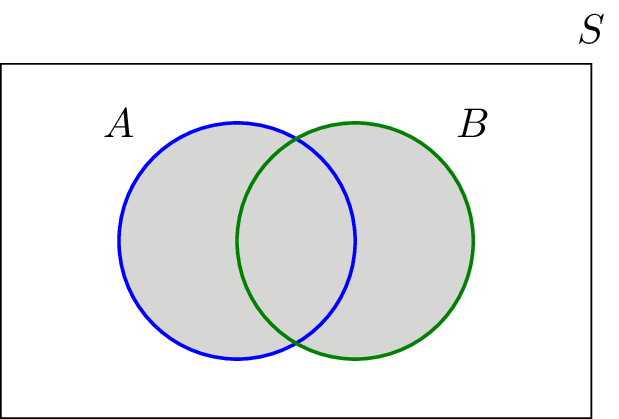
\includegraphics[width=1.5in,height=\textheight]{img/union_b.png}
      \caption{Unión de conjuntos}
      \end{minipage}%
      \begin{minipage}{0.5\linewidth}
      \centering
      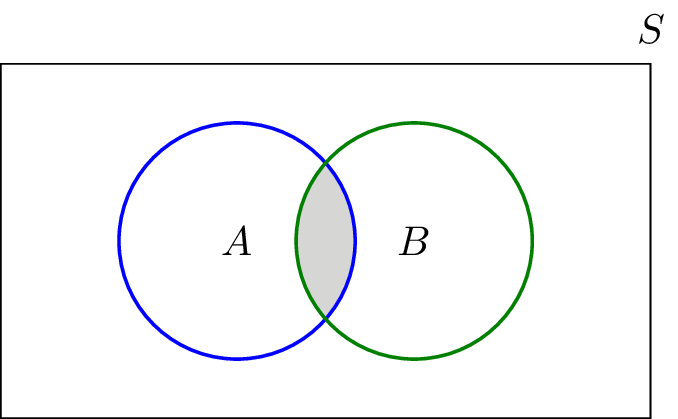
\includegraphics[width=1.5in,height=\textheight]{img/intersection_b.png}
      \caption{Intersección de conjuntos}
      \end{minipage}

      \begin{minipage}{0.5\linewidth}
      \centering
      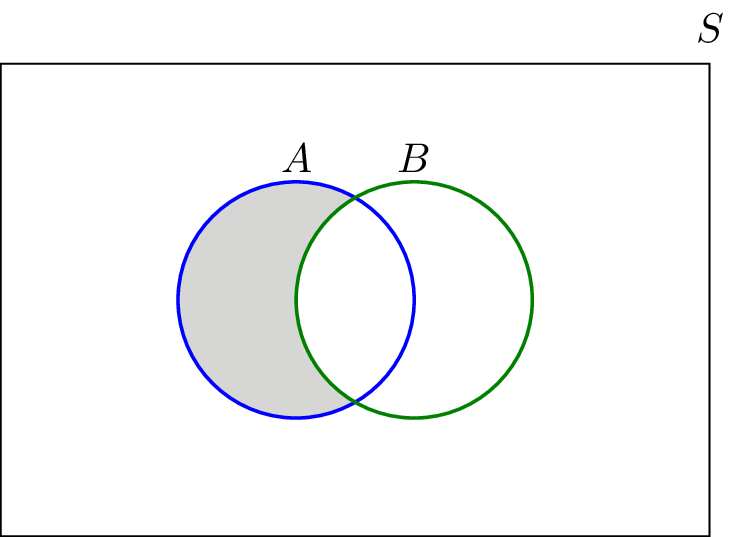
\includegraphics[width=1.5in,height=\textheight]{img/difference_b.png}
      \caption{Resta de conjuntos}
      \end{minipage}%
      \begin{minipage}{0.5\linewidth}
      \centering
      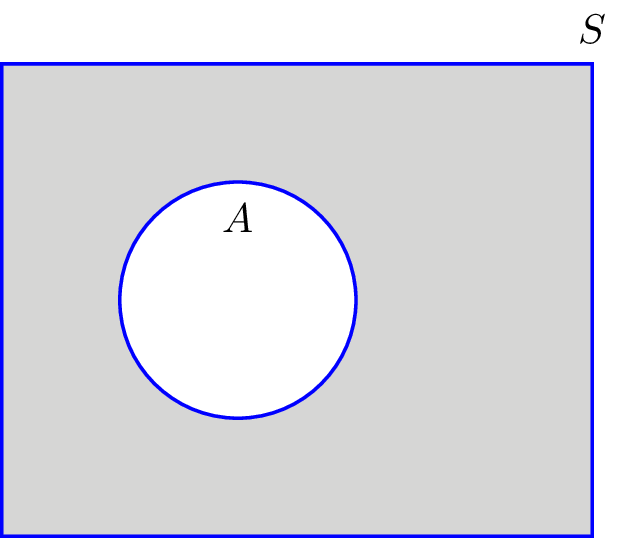
\includegraphics[width=1in,height=\textheight]{img/complement_b.png}
      \caption{Complementario de conjunto}
      \end{minipage}
    \end{figure} 
\end{note}


\newpage
\section{Definición de probabilidad y sus propiedades}

Definir de manera formal la probabilidad require conocimientos que se salen de lo que se intenta transmitir aquí. Daremos una aproximación
al concepto de probabilidad a través de sus propiedades.

A un nivel intuitivo, dado un experimento aleatorio y un suceso $A\in \Omega$, la \textbf{probabilidad} de $A$,
es un número entre $0$ y $1$ que denotaremos por $P(A)$ y que expresa 
\begin{itemize}
  \item la frecuencia relativa con la que se presenta el suceso (al repetir el experimento si esto fuera posible)
  \item la proporción o cociente entre el número de resultados que forma el suceso y el número de sucesos posibles del experimento.
  \item el grado de creencia o certeza que tenemos de la ocurrencia del suceso
\end{itemize}

La manera en que se define la propiedad es a través de sus axiomas, que son tres. Dado un espacio muestral $\Omega$, la probabilidad asigna a cada $A\in \Omega$ un número
$P(A)$ que cumple
\begin{enumerate}
  \item[i.] $P(A)$ está entre $0$ y $1$
  \item[ii.] $P(\Omega) = 1$
  \item[iii.] Si $A$ y $B$ son sucesos excluyentes (esto es, $A\cap B = \emptyset$) entonces $P(A\cup B) = P(A) + P(B)$.
\end{enumerate}

\end{document}